\documentclass[tikz,border=3.14mm]{standalone}
\begin{document}
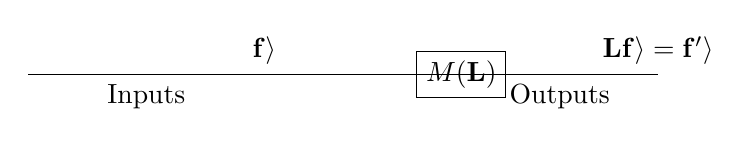
\begin{tikzpicture}
   \draw (-1.5,0) -- (1.5,0) node[midway,below] {Inputs} node[above] {$\lvert \mathbf{f} \rangle$};
   \draw (4,0) -- (6.5,0) node[midway,below] {Outputs} node[above] {$\mathbf{L}\lvert \mathbf{f} \rangle = \lvert \mathbf{f}' \rangle$};
   \node[draw,rectangle] at (4,0) (M) {$M(\mathbf{L})$};
   \draw (0,0) -- (4,0);
\end{tikzpicture}
\end{document}